\documentclass{homework}
\usepackage[utf8]{inputenc}
\usepackage{amsmath}
\usepackage{amssymb}
\usepackage{braket}
\usepackage{graphicx}
\newcommand{\hwname}{Vaansh Lakhwara}
\newcommand{\hwemail}{ID: 401147641}
\newcommand{\hwnum}{6}
\newcommand{\hwtype}{Assignment}
\newcommand{\hwclass}{COMP 335}
\begin{document}
\maketitle
\question
\textbf{(a)}
G${_1}$ = (V, T, S, P) such that V is a set of variables $\{S,X\}$, where S is the start variable and T is the set of terminals \{0,1\}.\\
S $\rightarrow$ XY\\
X $\rightarrow$ 0X0 | 1X1 | Y\\
Y $\rightarrow$ ZZ\\
Z $\rightarrow$ 0|1 \\
\newline
\textbf{(b)}
G${_2}$ = (V, T, S, P) such that V is a set of variables $\{S,X\}$, where S is the start variable and T is the set of terminals \{a,b,c,d\}.\\
S $\rightarrow$ aSc | aSd | X\\
X $\rightarrow$ bXc | bXd | $\lambda$\\
\newline
\textbf{(c)}
G${_3}$ = (V, T, S, P) such that V is a set of variables $\{S,X,Y\}$, where S is the start variable and T is the set of terminals \{a,b\}.\\
S $\rightarrow$ YXYaaYXY\\
X $\rightarrow$ XaXbX | XbXaX | $\lambda$\\
Y $\rightarrow$ aY | $\lambda$
\question
\textbf{(a)}
\newline
\begin{center}
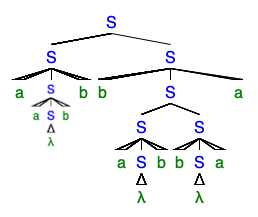
\includegraphics{a6q2a.png}
\end{center}
\newline
\textbf{(b)}
$S\Rightarrow SS$\\
\phantom{x}\hspace{4ex} $\Rightarrow aSbS$ \\
\phantom{x}\hspace{4ex} $\Rightarrow aaSbbS$ \\
\phantom{x}\hspace{4ex} $\Rightarrow aabbS$ \\
\phantom{x}\hspace{4ex} $\Rightarrow aabbbSa$ \\
\phantom{x}\hspace{4ex} $\Rightarrow aabbbSSa$ \\
\phantom{x}\hspace{4ex} $\Rightarrow aabbbaSbSa$ \\
\phantom{x}\hspace{4ex} $\Rightarrow aabbbabSa$ \\
\phantom{x}\hspace{4ex} $\Rightarrow aabbbabbSaa$ \\
\phantom{x}\hspace{4ex} $\Rightarrow aabbbabbaa$ \\
\newline
\textbf{(c)}
Yes, the grammar $G$ is ambiguous.\\
\textbf{Explanation:}
a CFG is said to be ambiguous iff there exists a string in T that has more than one parse tree representation.\\
\newline
Lets take string $abab$ for instance. The string exists in grammar $G$ it can be represented as the two parse trees as seen below (Tree 1 and Tree 2). Therefore, the grammar $G$ is ambiguous.\\
\newline
\begin{center}
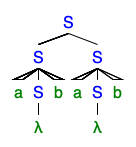
\includegraphics{a6q2c1.png}
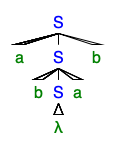
\includegraphics{a6q2c2.png}
\\
Tree 1 \quad \quad \quad \quad \quad \quad \quad  \quad \quad Tree 2
\end{center}
\end{document}